\chapter{研究概览}
\label{chp:dataCollection}

% \subsection{Workflow of Our Study}
\section{本文研究流程}

\begin{figure}[htbp]
	\centering
	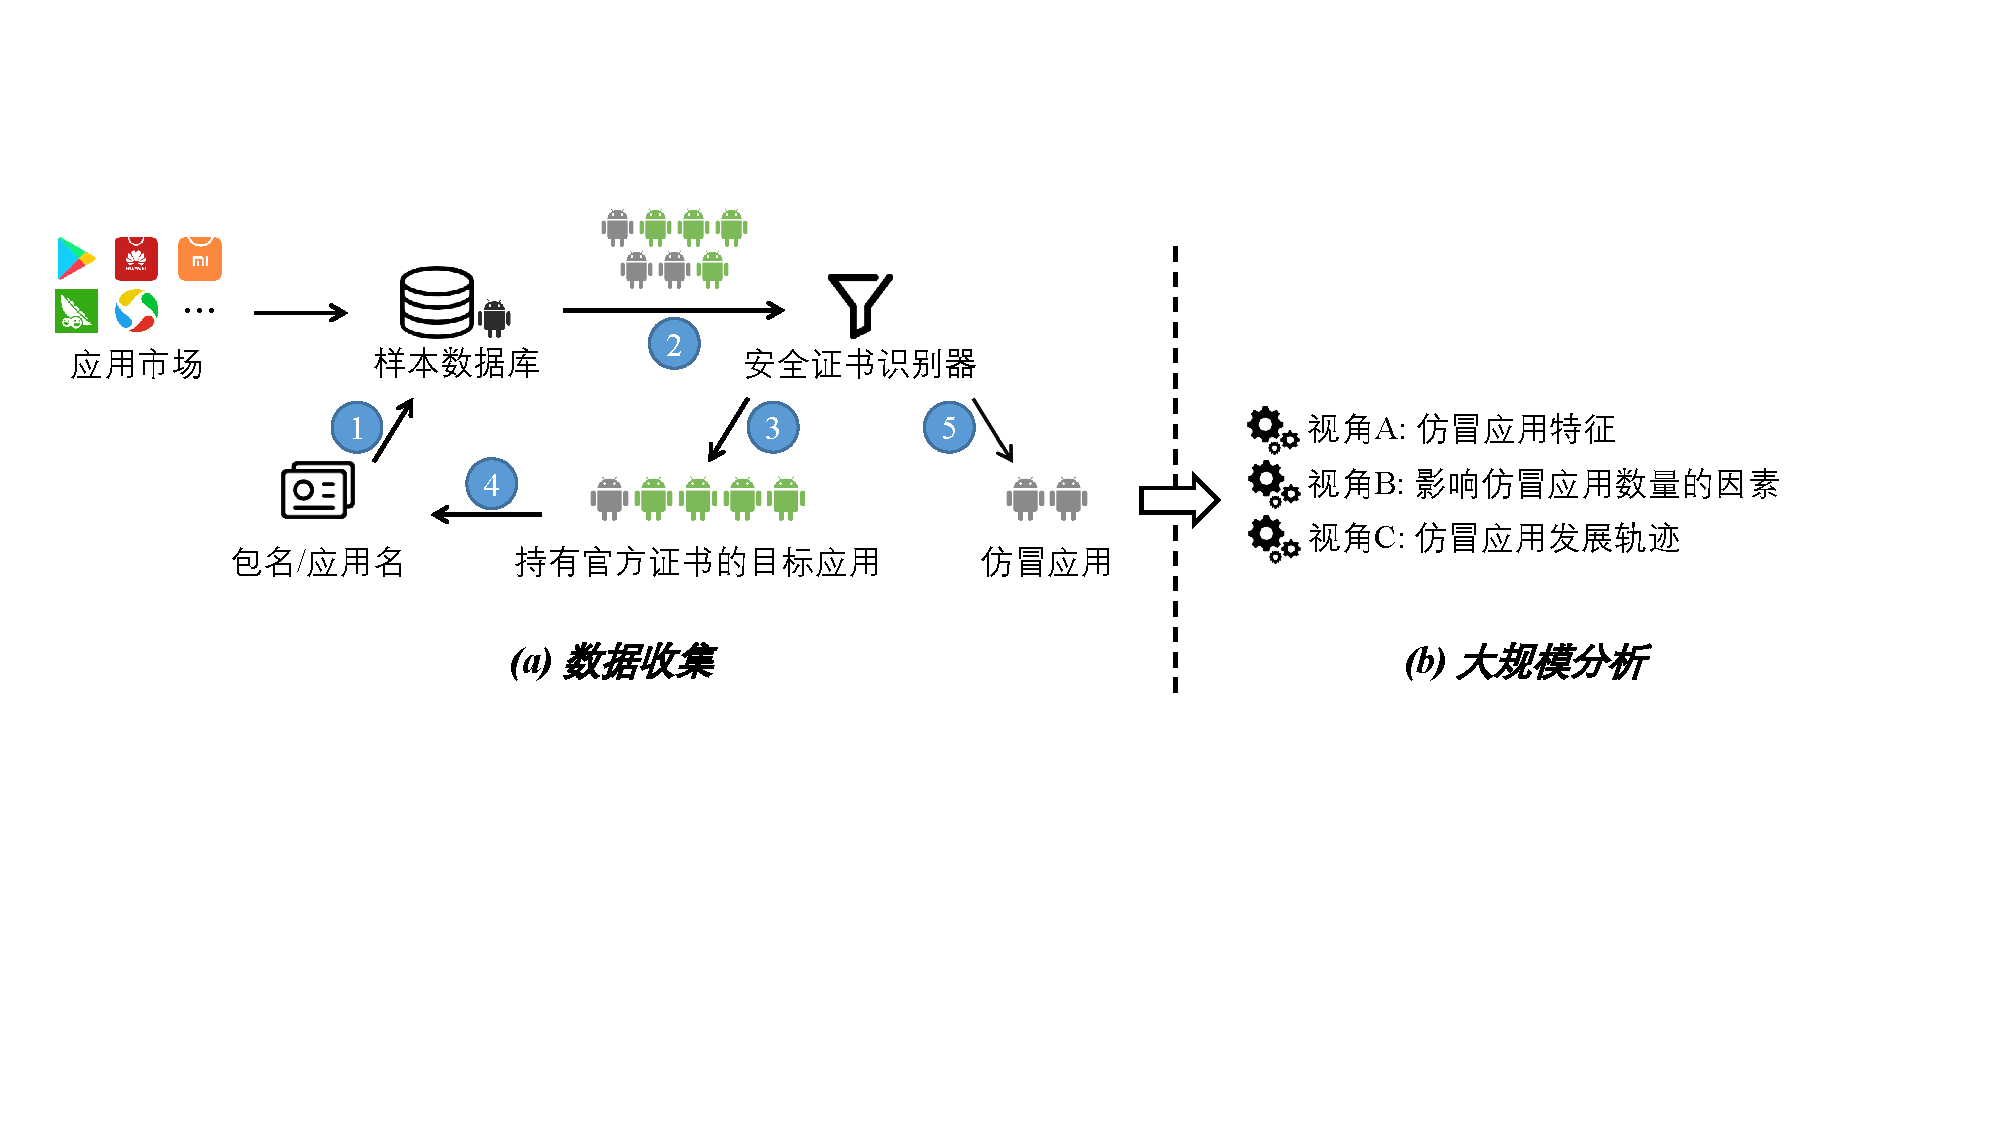
\includegraphics[width=0.95\textwidth]{./Figures/overview_modified.pdf}
	\caption{本文研究流程}
	\label{fig:Workflow}
	\vspace{-3mm}
\end{figure}

% Fig.~\ref{fig:Workflow} shows the workflow of our study, which can be divided into two main phases:
\autoref{fig:Workflow} 展示了\fullref{chp:discoveries}的工作流程,其可以分为两个主要阶段:

% (1)\ \emph{Data Collection}, which collects fake apps from all sorts of app markets based on the maintained official certificates, as well as the metadata of apps (e.g., package names and app names).
1)\ \emph{数据收集} \quad
在这一步,我们基于搜集到的官方应用安全证书的信息,从各大应用市场收集仿冒应用和他们的相关元数据(比如App的包名和应用名)。
% Our collaboration with \texttt{\small Pwnzen} allows us to have access to raw data from most of the mainstream Android markets.
得益于与上海犇众信息技术有限公司的合作,我们从Google Play官方应用商店和国内的大部分主流第三方应用市场中顺利收集到了大量的原始数据。

我们的研究对象是仿冒应用,但市面上的App林林总总,不可一概全收,一些小型的App相似度极高,更是难辨其原创性。
% We focus on collecting the fakes of the top 50 popular apps in the real world;
因此,我们在收集仿冒应用时,只收集了当时国内市面上最热门50款App的对应仿冒样本。
在选择市面上最热门的50款App时,我们参考了当时数据平台易观千帆的月度App排行榜\footnote{\url{https://qianfan.analysys.cn/refine/view/rankApp/rankApp.html}},然后从中选出了其中的前50款热门App,搜集它们的仿冒样本。

% 2)\ \emph{Large-scale Empirical Study}, which measures the collected fake apps from several perspectives: the characteristics of fake apps, as well as the quantitative analysis of fake apps.
2)\ \emph{大规模实证研究} \quad
在这一步,我们对搜集到的仿冒样本,从以下角度进行大规模的实证研究:仿冒的基本应用特征、针对仿冒应用的定量分析。
% We also aim to unveil the developing trend of fake authors to help fake app detection and shine light on the nature of the fake apps' ecosystem for both academia and industry.
我们也试图从收集到的信息中挖掘出仿冒应用作者的开发轨迹,以求为学术界和工业界揭示仿冒应用生态系统的更多信息。

在此之外,在\fullref{chp:feedback}中,我们还从几个第三方应用市场中随机选取一部分应用,提取了用户对它们的所有历史评价,然后筛选出其中对仿冒应用的评价并分析,以期了解用户对这些应用持有的态度,然后在此基础上检测仿冒应用是否有排名欺诈行为,为了方便作者理解,评论数据的收集、概览在\fullref{chp:feedback}另表。

% \section{Data Collection}
\section{数据收集}
% Although the research community is in great need of both a comprehensive dataset on Android fake apps from industry and an effective approach to retrieving and collecting fake apps at scale from industry, little has been done to fulfill the need.
尽管对于学术界来说,一个从市面上App收集的、完整而全面的仿冒应用数据集,又或是一套能大规模又有效地收集仿冒应用的方法会对相关研究十分有裨益,但是迄今为止,都未有相关工作能填补这一空白。
% In this paper, we make the first attempt to systematically collect data from industry.
因此,在本文中,我们率先尝试着从工业界中系统地收集我们需要的仿冒应用数据。

% \noindent {\bf Collection Method.}
\subsection{收集方法}
% Obtaining an ample set of data is a challenging task, new app samples and updates need to be continuously crawled from various Android markets.
% The challenge here is two-fold:
针对我们的研究主体,要获取足量的数据以组成数据集是一个十分具有挑战性的任务,难点主要有三:
\begin{itemize}
	% (1) Obtaining a large number of samples from different markets separately is no easy task;
	\item 我们要从多个不同的应用市场中爬取App样本,每个应用市场都有不同的网页编码,不存在一个爬虫脚本对所有应用市场数据都通用的场景;
	% (2) A certificate identifier is needed to tell fake apps from official ones.
	\item 各个应用市场架上的App数量浩如繁星,我们需要有效地找到和前述50个热门App有关的所有样本,不重不漏;
	\item 我们需要一个轻量级的解决方案快速判断获得的App样本究竟为正版应用又或者是仿冒应用。
\end{itemize}

% To address challenge (1), we collaborate with our industry partner and leverage the Pwnzen platform to conduct \emph{sample crawling} from markets and build a \texttt{\small sample database};
为了应对第一个挑战,我们与工业界合作,利用了犇众信息公司的Janus平台对各大应用商店进行\emph{样本爬取},然后用得到的样本构建了一个\texttt{\small 样本数据库}。
事实上,如\autoref{fig:Janus-data}显示,Janus平台自2017年起就开始对各大应用商店的App进行样本收集,至今已收集到上千万个App样本。
除样本搜集外,Janus也提供按规则搜索功能,用户可以创建自己的规则过滤平台中的应用数据,以获取自己需要的App样本。

\begin{figure}[htbp]
	\centering
	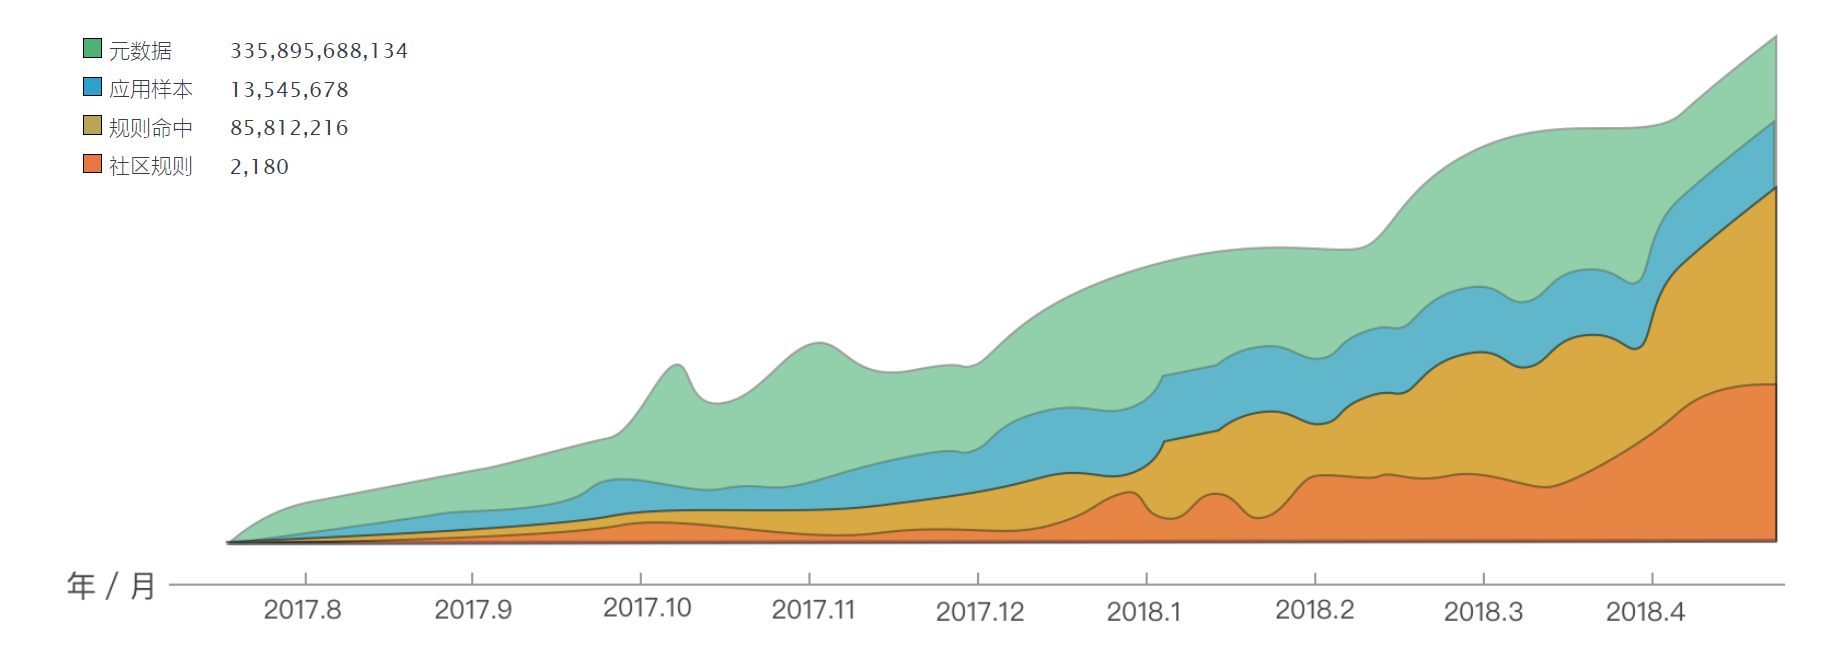
\includegraphics[width=\textwidth]{./Figures/edwin-Janus-data.png}
	\caption{Janus平台上的数据规模时序图}
	\label{fig:Janus-data}
	\vspace{-5mm}
\end{figure}

为了应对第二个挑战,我们使用了一个基于广度优先搜索(Breadth-First Search,简称BFS)的算法,分步搜索与50个热门应用相关的所有App样本,稍后会有详细介绍。

% to meet challenge (2), we pre-download the latest samples of our target apps to extract their official certificate information and construct a certificate identifier.
而为了应对第三个挑战,我们预先从官方渠道下载了50个热门应用的最新版本,提取出它们APK文件中包含的安全证书信息,构建出了一个安全证书筛选器。

% More specifically, during the database construction phase, we clusters samples by certificate hash, package names or app names.
更具体地说,在构建数据库的阶段,我们分别使用安全证书哈希码、App包名和App应用名来聚类应用样本。
% When the database receives queries, it returns sample clusters with the corresponding package names, app names, certificate hash, etc, in form of sample metadata entries.
当接收到查询请求时,数据库分别会返回与查询条目对应的包名、应用名和安全证书哈希码的聚类结果,结果以包含样本元数据的条目形式呈现。
% Since fake samples usually have similar names to the official ones, we collect fake apps by using app names from official apps.
为了迷惑用户,仿冒样本往往有与正版App十分相似的外观,比如与正版App近似的名称。
因此,我们以正版应用的应用名出发,搜寻仿冒应用。

% To achieve this, we first extract the package names of our pre-downloaded samples.
要做这件事,我们首先从预先下载好的正版样本APK文件中提取App的包名和应用名,放入查询队列中。
% These package names are later sent to the sample database for query (i.e., step 1 marked in Fig.~\ref{fig:Workflow}).
这些包名和应用名接下来会被输入到样本数据库中进行查询(即\autoref{fig:Workflow}中标识的步骤1)。
% And then, for each metadata entry returned from step 2, we check if it is official using the certificate identifier.
之后,数据库会返回一系列对应的样本结果(步骤2)。
对每个结果,我们会提取其中的安全证书哈希码字段,输入到安全证书识别器中,判定对应的样本是否持有正版应用的证书。
% If true and that sample is confirmed as one of our target app (step 3 in the figure), namely, it has the same package name to one of the inputs, its name will be recorded (step 4) and used for further query (back to step 1).
如果一个样本持有正版证书,它就会被认定为正版应用(图中的步骤3),我们会记录下它的包名和应用名(步骤4)。
如果它的包名(或应用名)还没有被用于查询过,我们会把这个包名(或应用名)加入查询队列,然后开始下一轮的迭代(回到步骤1)。
% If false, that sample would be marked as a fake one (step 5), its metadata will be utilized for large-scale measurement.
否则,这个样本会被标记成仿冒样本(图中步骤5)。
它的元数据将会被用于大规模分析。

之所以要这样操作,是因为开发者推出的App的应用名和包名并不是一成不变的。
一些热门应用会出于商业原因频繁地更改自己的应用名(比如爱奇艺视频,会根据其近期热播的电视剧/电影变更其应用名以吸引更多用户使用);
也有个别的热门应用可能会更换自己的包名,比如App有重大改版、又或者是开发者安全证书有变更,开发者不得不更换包名(具体原因可参考\secref{sec:signature}的Android App签名机制部分)。
% For each app, once all of the official names have been used for query, the data collection on it is finished.
对于每个热门应用来说,当其对应的查询队列中的所有包名、应用名都已经被查询过,我们对这个热门应用的数据收集就结束了。

% \noindent {\bf Collected Dataset.}
\subsection{数据概览}
% Here is a bird eye's view to the data we collected:
在这里,我们先给收集到的数据提供一个数据概览:

% we chose the top 50 popular apps from Analysys's ranking, within 11 app categories, as our target apps. Since apps may change their names over time,  we recorded 198 app names from the 50 apps to mine fake samples.
从易观千帆提供的数据榜单中,我们选择了50个最热门的App作为研究主体,这些App分属11个不同的应用类别。
由于App的应用名可能会在App更新迭代的时候随之变更,我们用近似BFS的策略,从50种App中一共记录了198个不同的应用名,来挖掘仿冒样本。
% Among the 50 apps, we failed to find any samples from the following three apps: \emph{OPPO AppStore}, \emph{Huawei AppStore}, and \emph{MI AppStore}, because they are developed by cellphone manufacturers and are not provided to other app markets.
在这50款App中,我们并不能在市面上找到以下三款App的任何样本:\emph{OPPO 应用商店},\emph{华为应用商店}和\emph{小米应用商店}。
因为这三款App都是由手机设备厂商开发和预装在对应品牌的手机中的,仅供这些品牌的用户使用,并不在其他应用市场上提供下载。
% This is also the reason why three apps are popular -- they are preinstalled into every single device produced by their manufacturers.
当然,这也是这三款App热度高的原因——这几款App都被预装到了对应手机品牌厂商的每一部Android设备中,而OPPO、华为和小米又是国内最大的几家手机厂商,这几款App自然也会有庞大的用户基数。
% Thus we finally obtained 47 target apps in total.
因此,我们最后的目标App只有47款。

% With the 47 target apps, we retrieve 138,106 distinct samples in total, 69,614 of which are official samples of our target apps, 52,638 samples lack registered certificates.
对这47款目标App,我们总共收集到了138,106个应用样本。
其中,69,614个应用样本持有官方开发者证书,52,638个应用样本并不具有官方证书。
还有一部分应用样本,是某些应用的分别发布在不同应用市场同一版本,在经过我们的去重筛选后被排除(共计15,854个)。

% For each sample, we retrieve 8 data items as metadata: \emph{Sample SHA1}, \emph{Certificate SHA1}, \emph{Package Name}, \emph{Package Size}, \emph{Version Number}, \emph{Retrieved Time}, and \emph{Source}.
对于每个样本,我们会收集8个数据项作为元数据:\emph{样本SHA1码},\emph{安全证书SHA1码},\emph{包名},\emph{样本大小},\emph{版本号},\emph{搜集时间}和\emph{APK包来源}。
% Among them, \emph{Sample SHA1} and \emph{Certificate SHA1} are the hash code for APK files and certificates under SHA1 algorithm respectively.
其中,\emph{样本SHA1码}是使用SHA1哈希算法对整个APK文件进行数据摘要之后获取到的编码串,每个样本都有独一无二的SHA1码;安全证书SHA1码则是对样本的安全证书采用SHA1算法提取数据摘要之后获取的编码串,用于识别不同的证书。
% \emph{Retrieve Time} tells when the sample was crawled from app store and \emph{Source} tells which store the sample is from.
而\emph{搜集时间}则是样本从应用市场被爬取到数据库的时间点,\emph{APK包来源}指示该APK包来源的应用市场。

\section{本章小结}

本章主要对本研究进行了概览,并详细介绍了数据收集的流程和方法,然后对采集到的数据进行了简要描绘。
% Empirical study is then applied to these metadata, especially to those of fake apps, to gain us a more comprehensive understanding on fake apps' nature and characteristics, and the behaviors of fake app authors.
接下来我们将针对前述的元数据,尤其是对仿冒样本中采集到的元数据,进行实证研究,以求获得对于仿冒应用生态和特征、以及对于仿冒应用开发者的行为的更全面的认知。
